\documentclass[12pt]{article}

% ----------------------------------------------------------------------
% Define external packages, language, margins, fonts, new commands 
% and colors
% ----------------------------------------------------------------------
\usepackage[utf8]{inputenc} % Codification
\usepackage[english]{babel} % Writing idiom

\usepackage{listings}
\usepackage[dvipsnames]{xcolor}
\usepackage[most]{tcolorbox}
\usepackage{float}


\definecolor{codebg}{RGB}{245,245,245}
\definecolor{codeframe}{RGB}{200,200,200}

\lstdefinestyle{CiscoStyle}{
    backgroundcolor=\color{codebg},
    basicstyle=\ttfamily\small,
    keywordstyle=\color{blue},
    commentstyle=\color{gray},
    breaklines=true,
    showstringspaces=false,
    columns=fullflexible
}

\newtcblisting{configbox}{
    listing only,
    colback=codebg,
    colframe=codeframe,
    arc=3mm,
    boxrule=0.5pt,
    left=2mm,
    right=2mm,
    top=1mm,
    bottom=1mm,
    listing options={style=CiscoStyle}
}

\newtcblisting{largeconfigbox}{
    listing only,
    breakable,
    colback=codebg,
    colframe=codeframe,
    arc=3mm,
    boxrule=0.5pt,
    listing options={
        style=CiscoStyle,
        basicstyle=\ttfamily\scriptsize
    }
}

\usepackage{graphicx}
\usepackage[export]{adjustbox} % Align images
\usepackage{amsmath} % Extra commands for math mode
\usepackage{amssymb} % Mathematical symbols
\usepackage{anysize} % Personalize margins
    \marginsize{2cm}{2cm}{2cm}{2cm} % {left}{right}{above}{below}
\usepackage{appendix} % Appendices
\usepackage{cancel} % Expression cancellation
\usepackage{caption} % Captions
    \captionsetup{labelfont={bf}}
\usepackage{cite} % Citations, like [1 - 3]
\usepackage{color} % Text coloring
\usepackage{fancyhdr} % Head note and footnote
    \pagestyle{fancy}
    \fancyhf{}
    \fancyhead[L]{\footnotesize IST} % Left of Head note
    \fancyhead[R]{\footnotesize ULisboa} % Right of Head note
    \fancyfoot[L]{\footnotesize DDRS} % Left of Footnote
    \fancyfoot[C]{\thepage} % Center of Footnote
    \fancyfoot[R]{\footnotesize METI} % Right of Footnote
    \renewcommand{\footrulewidth}{0.4pt} % Footnote rule
\usepackage{float} % Utilization of [H] in figures
\usepackage{graphicx} % Figures in LaTeX
\usepackage[colorlinks = true, plainpages = true, linkcolor = istblue, urlcolor = istblue, citecolor = istblue, anchorcolor = istblue]{hyperref}
\usepackage{indentfirst} % First paragraph
\usepackage[super]{nth} % Superscripts
\usepackage{siunitx} % SI units
\usepackage{subcaption} % Subfigures
\usepackage{titlesec} % Font
    \titleformat{\section}{\Large\bfseries}{\thesection}{1em}{}
    \titleformat{\subsection}{\large\bfseries}{\thesubsection}{1em}{}
    \titleformat{\subsubsection}{\normalsize\bfseries}{\thesubsubsection}{1em}{}
    \fancyfoot[C]{\thepage}

% New and re-newcommands
\newcommand{\sen}{\operatorname{\sen}} % Sine function definition
\newcommand{\HRule}{\rule{\linewidth}{0.5mm}} % Specific rule definition
\renewcommand{\appendixpagename}{\LARGE Appendices}

% Colors
\definecolor{istblue}{RGB}{3, 171, 230}
\definecolor{dkgreen}{rgb}{0,0.6,0}
\definecolor{gray}{rgb}{0.5,0.5,0.5}

%%%%%%%%%%%%%%%%%%%%%%%%%%%%%%%%%%%%%%%%%%%%%%%%%%%%%%%%%%%%%%%%%%%%%%%%
%                                 Document                             %
%%%%%%%%%%%%%%%%%%%%%%%%%%%%%%%%%%%%%%%%%%%%%%%%%%%%%%%%%%%%%%%%%%%%%%%%

\begin{document}

% ----------------------------------------------------------------------
% Cover
% ----------------------------------------------------------------------
\begin{center}
    \begin{figure}
        \vspace{-1.0cm}
        
\includegraphics[scale = 0.1, left]{../images/IST_A.png} % IST logo
    \end{figure}
    \mbox{}\\[2.0cm]
    \textsc{\Huge Performance Evaluation and Dimensioning of Networks and Systems}\\[2.5cm]
    \textsc{\LARGE METI}\\[2.0cm]
    \HRule\\[0.4cm]
    {\large \bf {Lab 1 Report} [\texttt{EN}]}\\[0.2cm]
    \HRule\\[1.5cm]
\end{center}

\begin{flushleft}
    \textbf{Authors:}
\end{flushleft}

\begin{center}
    \begin{minipage}{0.5\textwidth}
        \begin{flushleft}
            José Oliveira (103771) \\
            Afonso Mendes (116024) \\
            Tiago Videira (116069)
        \end{flushleft}
    \end{minipage}%
    \begin{minipage}{0.5\textwidth}
        \begin{flushright}
            \href{mailto:jose.novais.oliveira@tecnico.ulisboa.pt}{\texttt{jose.novais.oliveira@tecnico.ulisboa.pt}}\\
            \href{mailto:afonsofmendes@tecnico.ulisboa.pt}{\texttt{afonsofmendes@tecnico.ulisboa.pt}}\\
            \href{mailto:tiago.g.videira@tecnico.ulisboa.pt}{\texttt{tiago.g.videira@tecnico.ulisboa.pt}}\\
        \end{flushright}
    \end{minipage}
\end{center}

\vspace{1.2cm}
\begin{center}
    \large \bf 2026/2027 -- \nth{1} Semester
\end{center}

\thispagestyle{empty}
\setcounter{page}{0}
\newpage

% ----------------------------------------------------------------------
% Contents
% ----------------------------------------------------------------------
\tableofcontents 
\newpage

% ----------------------------------------------------------------------
% Body
% ----------------------------------------------------------------------

% ======================================================================
\section{Introduction}
% ======================================================================

This report documents the work developed for Laboratory~1 of the Performance Evaluation and Dimensioning of Networks and Systems (DDRS) course, covering the fourteen exercises proposed in the laboratory guide. The exercises progress from the fundamentals of random number generation to the construction and analysis of discrete-event simulators, and finally to statistical techniques for validating and interpreting simulation output.

The report follows the same structure as the laboratory guide, organized into six parts. Part~A covers the properties of R's pseudo-random number generator. Part~B addresses the generation of random variables and stochastic processes -- Bernoulli and exponential random variables, and Poisson arrival processes -- from a uniform random number generator. Part~C develops discrete-event simulators for the M/M/1 and M/M/2 queuing systems and compares their output against the corresponding theoretical performance metrics. Part~D estimates a probability through Monte Carlo simulation. Part~E applies statistical tools -- histograms, confidence intervals, and an assessment of confidence-interval coverage -- to both real network measurements (packet captures and RTT measurements) and synthetic data. Part~F examines practical aspects of simulation output analysis: run-to-run variability, the effect of initial conditions, and the replication/deletion procedure for determining an adequate number of replications.

For each exercise, the report states the objective, describes the approach and the corresponding R script, and presents the results together with a discussion of what can be concluded from them. All scripts were developed in R and executed in RStudio; network traffic was captured with Wireshark.

\newpage

% ======================================================================
\section{A. Random number generators}
% ======================================================================

\subsection{Exercise 1}

\textbf{Objective:} Generate 10000 random numbers uniformly distributed in $[0,1]$ using \texttt{runif()} and plot their histogram with \texttt{hist()}, to check informally whether the generator behaves as expected.

\textbf{Approach:} The following R script generates the sample and plots the histogram.

\begin{configbox}
numbers <- runif(10000, min = 0, max = 1)
hist(numbers, main = "Histogram", xlab = "Value", ylab = "Samples",
     col = "lightblue", border = "black")
\end{configbox}

\begin{figure}[H]
    \centering
    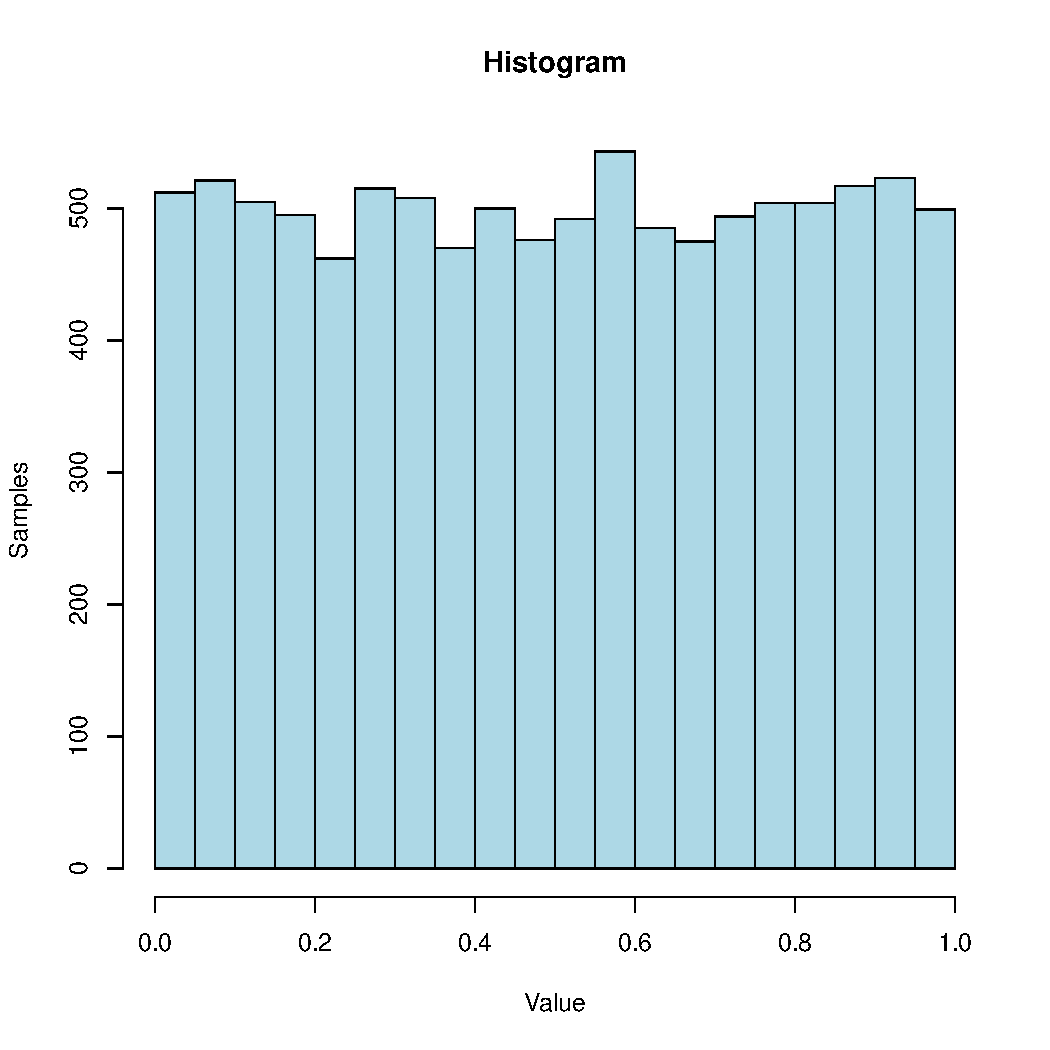
\includegraphics[width=0.6\textwidth]{../images/E1_Histogram.pdf}
    \caption{Histogram of 10000 samples generated with \texttt{runif()}.}
    \label{fig:ex1_hist}
\end{figure}

\textbf{Conclusion:} As shown in Figure~\ref{fig:ex1_hist}, the samples are approximately evenly distributed across all bins in $[0,1]$, with no systematic bias toward any sub-interval. This is consistent with the expected behavior of a uniform distribution, confirming that \texttt{runif()} is generating numbers as intended.

\subsection{Exercise 2}

\textbf{Objective:} Verify, using \texttt{runif()}, that the sequence generated by a pseudo-random number generator is in fact deterministic, i.e., that it can be reproduced exactly.

\textbf{Approach:} The \texttt{set.seed()} function fixes the internal state of R's random number generator. By setting the same seed before two separate calls to \texttt{runif()}, the two resulting sequences can be compared with \texttt{identical()} to check whether they match exactly. As a control, a third sequence is generated without resetting the seed, so it is expected to differ.

\begin{configbox}
set.seed(123)
seq1 <- runif(5)

seq_random <- runif(5)   # generated without resetting the seed

set.seed(123)
seq2 <- runif(5)

identical(seq1, seq2)
\end{configbox}

\begin{figure}[H]
    \centering
    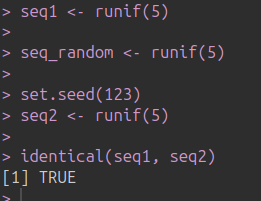
\includegraphics[width=0.3\textwidth]{../images/E2_Deterministic.png}
    \caption{R console output confirming that \texttt{seq1} and \texttt{seq2} are identical.}
    \label{fig:ex2_console}
\end{figure}

\textbf{Conclusion:} As shown in Figure~\ref{fig:ex2_console}, \texttt{identical(seq1, seq2)} returns \texttt{TRUE}, confirming that \texttt{seq1} and \texttt{seq2} are exactly the same sequence, even though they were generated by separate calls to \texttt{runif()}. This happens because \texttt{set.seed()} resets the internal state of the generator to the same fixed value before each call, so the pseudo-random number generator produces identical output whenever it starts from the same seed. This demonstrates that the sequence is not truly random but deterministic, fully determined by the seed. In contrast, \texttt{seq\_random}, generated without resetting the seed, follows on from the generator's state after \texttt{seq1} and therefore differs from both.

% ======================================================================
\section{B. Generation of random variables and stochastic processes}
% ======================================================================

\subsection{Exercise 3}

\textbf{Objective:} Develop an R script to generate Bernoulli distributed numbers from a uniform random number generator (\texttt{runif()}), and plot a histogram of 1000 samples to informally check that the generator behaves correctly.

\textbf{Approach:} A Bernoulli random variable with success probability $p$ can be generated from a uniform random variable $U \sim \text{Unif}(0,1)$ by setting the outcome to 1 if $U < p$ and 0 otherwise, using the \texttt{ifelse()} function. Here $p = 0.7$ and $n = 1000$ samples were generated.

\begin{configbox}
p <- 0.7            # success probability
n_samples <- 1000   # number of samples

u <- runif(n_samples)

bernoulli_numbers <- ifelse(u < p, 1, 0)

hist(bernoulli_numbers, 
     breaks = c(-0.5, 0.5, 1.5), 
     main = "Bernoulli Numbers Histogram (p = 0.7)", 
     xlab = "Outcome", 
     ylab = "Frequency",
     col = "lightblue", 
     xaxt = "n")
  
axis(1, at = c(0, 1))
\end{configbox}

\begin{figure}[H]
    \centering
    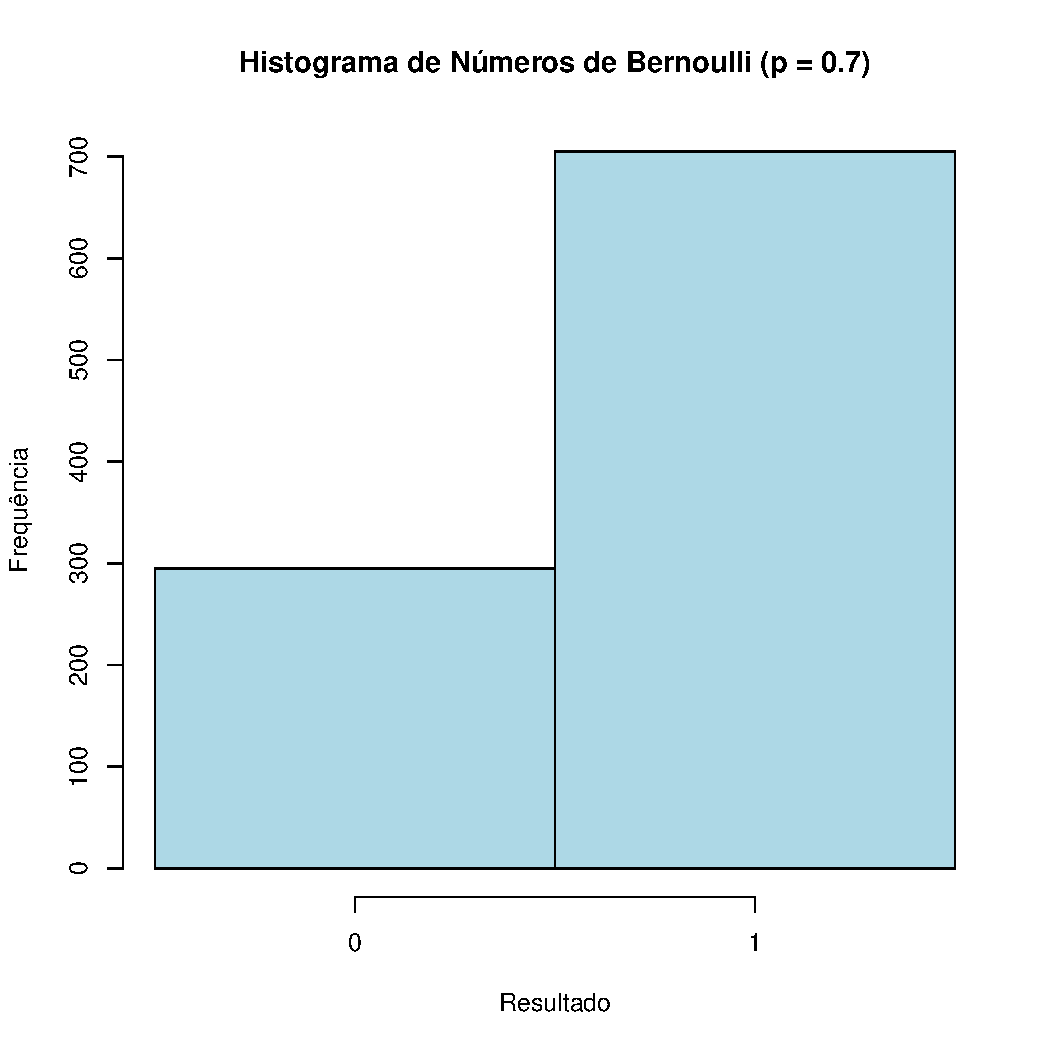
\includegraphics[width=0.6\textwidth]{../images/E3_Bernoulli.pdf}
    \caption{Histogram of 1000 Bernoulli samples with $p = 0.7$.}
    \label{fig:ex3_bernoulli}
\end{figure}

\textbf{Conclusion:} As shown in Figure~\ref{fig:ex3_bernoulli}, out of 1000 samples approximately 700 outcomes are 1 and 300 are 0, matching the expected proportions for $p = 0.7$. This confirms that thresholding a uniform random variable at $p$ is a valid method for generating Bernoulli distributed samples, since $P(U < p) = p$ for $U \sim \text{Unif}(0,1)$.

\subsection{Exercise 4}

\textbf{Objective:} Develop an R script to generate exponentially distributed numbers from a uniform random number generator (\texttt{runif()}), and plot a histogram of 10000 samples superposed with the theoretical pdf, to informally check that the generator behaves correctly.

\textbf{Approach:} Exponentially distributed samples can be generated from a uniform random variable $U \sim \text{Unif}(0,1)$ via the inverse transform method: since the exponential CDF is $F(x) = 1 - e^{-\lambda x}$, setting $U = F(X)$ and solving for $X$ gives $X = -\ln(1-U)/\lambda$. The histogram is plotted with \texttt{prob=TRUE} so that its area is normalized to 1, making it directly comparable to the theoretical pdf obtained with \texttt{dexp()}, which is superposed using \texttt{lines()}. Here $\lambda = 1.5$ and $n = 10000$ samples were generated.

\begin{configbox}
lambda <- 1.5        # rate of the exponential distribution
n_samples <- 10000   # number of samples

u <- runif(n_samples)
exp_numbers <- -log(1 - u) / lambda

hist(exp_numbers, 
     breaks = 50, 
     prob = TRUE, 
     main = "Exponential Distribution (lambda = 1.5)", 
     xlab = "Value", 
     ylab = "Density",
     col = "lightgray", 
     border = "white")

x_vals <- seq(0, max(exp_numbers), length.out = 500)
pdf_vals <- dexp(x_vals, rate = lambda)

lines(x_vals, pdf_vals, col = "red", lwd = 2)
\end{configbox}

\begin{figure}[H]
    \centering
    \begin{subfigure}{0.48\textwidth}
        \centering
        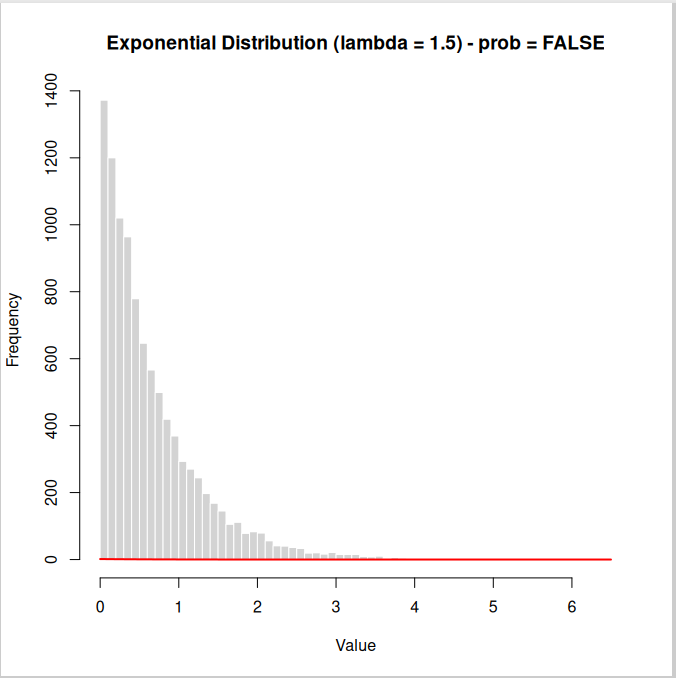
\includegraphics[width=\textwidth]{../images/E4_pdfExpoDistribution_notnorm.png}
        \caption{\texttt{prob = FALSE}}
        \label{fig:ex4_notnorm}
    \end{subfigure}
    \hfill
    \begin{subfigure}{0.48\textwidth}
        \centering
        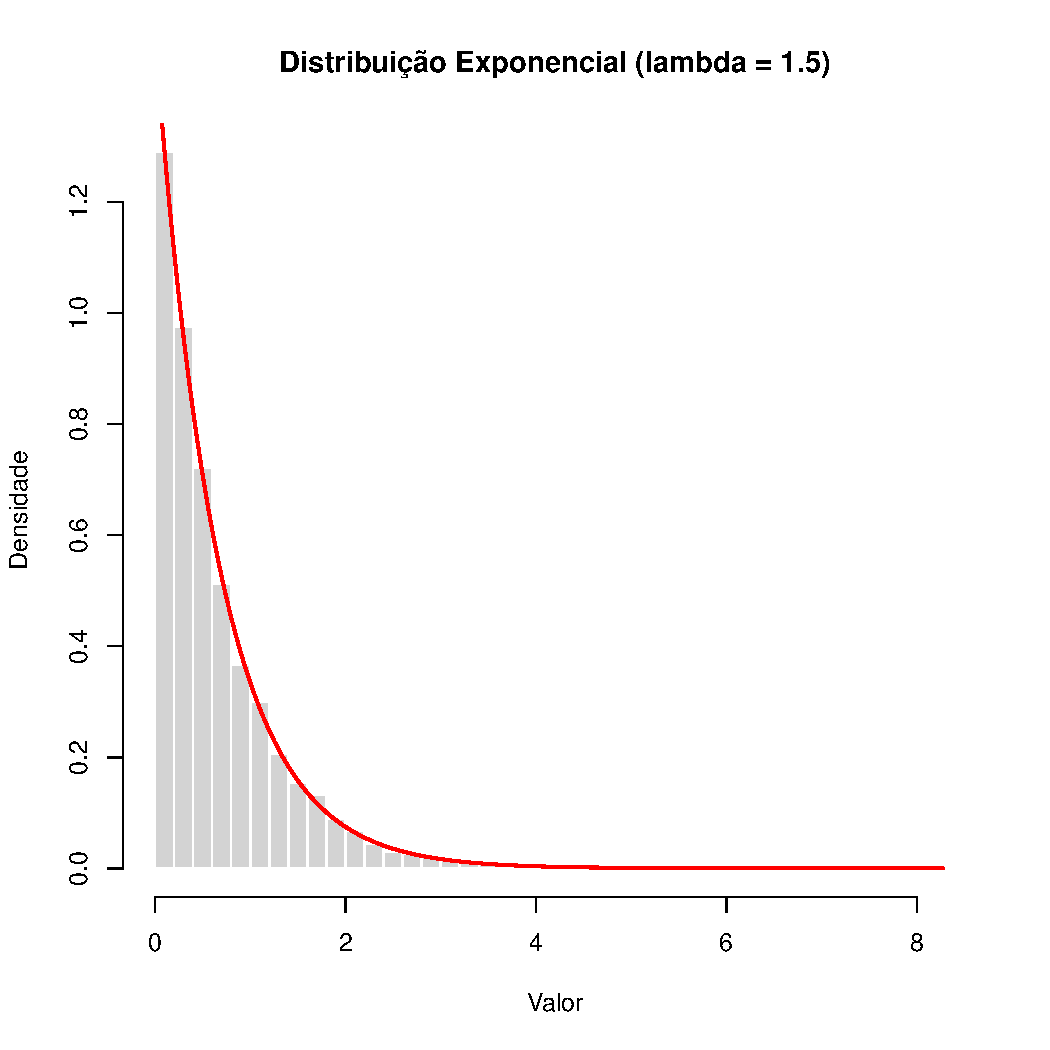
\includegraphics[width=\textwidth]{../images/E4_pdfExpoDistribution.pdf}
        \caption{\texttt{prob = TRUE}}
        \label{fig:ex4_norm}
    \end{subfigure}
    \caption{Histogram of 10000 exponentially distributed samples ($\lambda = 1.5$) with the theoretical pdf (red line) superposed, with and without density normalization.}
    \label{fig:ex4_exp}
\end{figure}

\textbf{Conclusion:} Figure~\ref{fig:ex4_exp} shows why the \texttt{prob=TRUE} option is essential for this comparison. In Figure~\ref{fig:ex4_notnorm} (\texttt{prob=FALSE}), the histogram bars represent raw counts per bin, whose total sums to $n = 10000$, while the \texttt{dexp()} curve has area 1 by definition; the two are on completely different scales, so the pdf line appears flat against the axis and gives no useful comparison. In Figure~\ref{fig:ex4_norm} (\texttt{prob=TRUE}), the histogram is rescaled so that the total area of the bars is also 1, matching the normalization of the theoretical pdf, and the empirical histogram now closely follows the red curve. This confirms that the inverse transform method correctly generates exponentially distributed samples from uniform random numbers, and that density normalization is a necessary condition for a visual histogram-vs-pdf comparison to be meaningful.

\subsection{Exercise 5}

\textbf{Objective:} Develop an R script to generate the arrival times of a Poisson process, and perform a simple test to verify that the sample rate matches the population rate.

\textbf{Approach:} A Poisson process with rate $\lambda$ has exponentially distributed inter-arrival times with parameter $\lambda$. Thus, inter-arrival times can be generated directly with \texttt{rexp()}, and the arrival times are obtained by accumulating them with \texttt{cumsum()}. To verify the generator, the sample rate is estimated from the generated data and compared with the population rate $\lambda$ used to generate it.

\begin{configbox}
lambda <- 2.0         
n_arrivals <- 10000

inter_arrival_times <- rexp(n_arrivals, rate = lambda)

arrival_times <- cumsum(inter_arrival_times)

estimated_lambda <- 1/mean(inter_arrival_times)

cat("Population rate (lambda):", lambda, "\n")
cat("Estimated rate (sample):", estimated_lambda, "\n")

head(arrival_times, 10)
\end{configbox}

\begin{figure}[H]
    \centering
    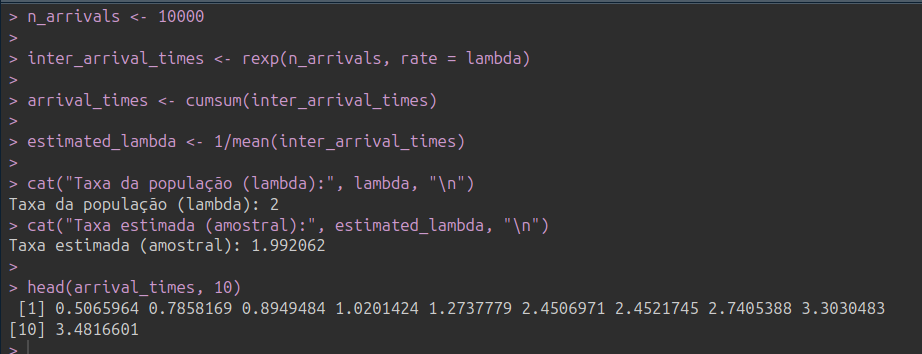
\includegraphics[width=0.7\textwidth]{../images/E5_Console.png}
    \caption{R console output showing the population rate, the estimated rate, and the first 10 arrival times.}
    \label{fig:ex5_console}
\end{figure}

\textbf{Conclusion:} As shown in Figure~\ref{fig:ex5_console}, with a population rate of $\lambda = 2$, the estimated rate from the sample is $\hat{\lambda} \approx 1.992$, very close to the true value. This result follows directly from the definition of $\lambda$: it represents the average number of arrivals per unit time, i.e., the rate of the process. Its reciprocal, $1/\lambda$, is the mean time between consecutive arrivals -- the expected value of the exponential inter-arrival time distribution, $E[T] = 1/\lambda$. Since the sample mean of the generated inter-arrival times, $\overline{T}$, is an estimator of $E[T]$, taking its reciprocal, $1/\overline{T}$, naturally produces an estimator of $\lambda$ itself. In other words, $\lambda$ measures "events per unit time" while $E[T]$ measures "time per event", so the two quantities are inverses of each other by construction, and computing $1/\overline{T}$ recovers an estimate of the rate that generated the data. The close agreement between $\hat{\lambda}$ and $\lambda$ confirms that the inter-arrival times were correctly generated as exponentially distributed with rate $\lambda$.

% ======================================================================
\section{C. Programming discrete event simulators}
% ======================================================================

\subsection{Exercise 6}

\textbf{Objective:} Modify the M/M/1 simulator of Annex A to also estimate the average delay in system and the server utilization, and compare the results against the theoretical values (Annex B), for at least two values of $\lambda/\mu$ with $\lambda/\mu < 1$.

\textbf{Approach:} Starting from the simulator in Annex A, the following changes were made to also track the average delay in system and the server utilization, in addition to the average delay in queue already computed by the original code:

\begin{itemize}
    \item State variables were added to accumulate customers' time in the system and to measure the intervals during which the server is busy.
    \item At the very start of each loop iteration, right after \texttt{Time} is updated and \emph{before} branching on the event type, the interval since the last event is added to \texttt{BusyTime} if the server was busy during that interval. This must be done unconditionally for both arrivals and departures, since the server can remain busy across either type of event:
    \begin{configbox}
NextEventType=which.min(EventList)
Time=EventList[NextEventType]
if (ServerStatus==1) {                    # NEW
  BusyTime=BusyTime+(Time-LastEventTime)  # NEW
}                                          # NEW
LastEventTime=Time                        # NEW
    \end{configbox}
    \item In the arrival branch, when the server is free, the customer's arrival time is stored in \texttt{InServiceArrivalTime} (as before):
    \begin{configbox}
ServerStatus=1
InServiceArrivalTime=Time          # NEW
EventList[2]=Time+rexp(1,ServiceRate)
    \end{configbox}
        \item On departure, the customer's time in the system is accumulated. If another customer is waiting, its arrival time is stored when service begins:
    \begin{configbox}
AcumSystemTime=AcumSystemTime+
    Time-InServiceArrivalTime
NumQueueCompleted=NumQueueCompleted+1
if (NumInQueue==0) {
  ServerStatus=0
  EventList[2]=Inf
} else {
  AcumDelay=AcumDelay+Time-QueueArrivalTime[1]
    InServiceArrivalTime=QueueArrivalTime[1]
  QueueArrivalTime=QueueArrivalTime[-1]
  NumInQueue=NumInQueue-1
  EventList[2]=Time+rexp(1,ServiceRate)
}
    \end{configbox}
    \item After the loop, the average delay in system and the server utilization are computed alongside the average delay in queue:
    \begin{configbox}
AvgDelay=AcumDelay/NumQueueCompleted
AvgTimeInSystem=AcumSystemTime/NumQueueCompleted   # NEW
Utilization=BusyTime/Time                          # NEW
    \end{configbox}
\end{itemize}

The simulation was run with $\text{NumQueueCompleted}=100000$ for three stable configurations ($\lambda/\mu<1$) and, for comparison, one critically loaded configuration ($\lambda/\mu=1$), with a fixed random seed (\texttt{set.seed(6)}) for reproducibility. The theoretical values were computed from Annex B: $W_Q = \dfrac{\lambda}{\mu(\mu-\lambda)}$, $W = \dfrac{1}{\mu-\lambda}$, and $\rho = \lambda/\mu$.

\begin{table}[H]
\centering
\begin{tabular}{|c|c|c|c|c|c|c|c|c|}
\hline
$\lambda$ & $\mu$ & $W_Q$ (sim.) & $W_Q$ (theo.) & $W$ (sim.) & $W$ (theo.) & $\rho$ (sim.) & $\rho$ (theo.) \\
\hline
1 & 2 & 0.5052 & 0.5000 & 1.0042 & 1.0000 & 0.4989 & 0.5000 \\
1 & 3 & 0.1705 & 0.1667 & 0.5036 & 0.5000 & 0.3334 & 0.3333 \\
1 & 4 & 0.0836 & 0.0833 & 0.3330 & 0.3333 & 0.2491 & 0.2500 \\
\hline
2 & 2 & 67.6446 & $\infty$ & 68.1427 & $\infty$ & 0.9951 & 1.0000 \\
\hline
\end{tabular}
\caption{Simulated vs. theoretical average delay in queue ($W_Q$), average delay in system ($W$), and server utilization ($\rho$), for different $\lambda/\mu$ ratios, with $\text{NumQueueCompleted}=100000$.}
\label{tab:ex6_results}
\end{table}

\textbf{Conclusion:} As shown in Table~\ref{tab:ex6_results}, for all stable configurations ($\rho<1$) the simulated $W_Q$, $W$, and $\rho$ now match the theoretical values predicted by the M/M/1 formulas very closely, with remaining discrepancies smaller than 1\%. Both the delays and the utilization increase as $\lambda/\mu$ approaches 1: for the M/M/1 system, $\rho=\lambda/\mu$ is precisely the theoretical fraction of time the server is busy, and this matches almost exactly against \texttt{BusyTime/Time} measured directly from the simulated trajectory. The last row ($\lambda=\mu=2$, $\rho=1$) illustrates the boundary of stability: the theoretical delays are infinite in the steady state, since the system is critically loaded (arrivals occur, on average, as fast as they can be served), and the simulated delay grows accordingly with the length of the run -- rising from about 3.4 with 1000 completed customers to 67.6 with 100000, while the utilization stays essentially at 1 (0.9951). This finite but growing delay is not a valid estimate of a steady-state quantity; rather, it confirms that at $\rho=1$ the queue has no stationary distribution and keeps building up indefinitely as the simulation runs longer, which is consistent with the theoretical divergence of $W_Q$ and $W$ as $\rho\to1$. This confirms that the condition $\rho<1$ required by the exercise is essential for the M/M/1 system to reach a stable steady state, and shows that server utilization, unlike the mean queuing delay, remains a well-defined and finite quantity even at the stability boundary.

\subsection{Exercise 7}

\textbf{Objective:} Develop a simulator for estimating the average delay in queue of an M/M/2 system, and compare the results with the theoretical values (Annex C), for at least two values of $\lambda/(2\mu)$ with $\lambda/(2\mu)<1$.

\textbf{Approach:} The M/M/1 simulator of Annex A was extended to two parallel servers. The key changes are: \texttt{ServerStatus} becomes a length-2 vector (one entry per server), and the event list has three entries instead of two -- one for arrivals and one departure event per server. On arrival, if both servers are busy the customer joins the queue; otherwise the customer is assigned to the first free server found with \texttt{which(ServerStatus==0)[1]}. On a departure, the freed server either goes idle (if the queue is empty) or immediately picks up the next customer in queue, and the corresponding delay is accumulated exactly as in the M/M/1 case.

\begin{configbox}
set.seed(7)
ArrivalRate=1
ServiceRate=2
Time=0
NumQueueCompleted=0
ServerStatus=c(0,0)          # 0 = idle, 1 = busy, one entry per server
NumInQueue=0
AcumDelay=0
QueueArrivalTime=c()
EventList=c(rexp(1,ArrivalRate), Inf, Inf)  # [arrival, dep@server1, dep@server2]

while (NumQueueCompleted<100000) {
  NextEventType=which.min(EventList)
  Time=EventList[NextEventType]

  if (NextEventType==1) {                    # ARRIVAL
    EventList[1]=Time+rexp(1,ArrivalRate)
    if (all(ServerStatus==1)) {               # both servers busy -> join queue
      QueueArrivalTime=c(QueueArrivalTime,Time)
      NumInQueue=NumInQueue+1
    } else {                                  # a server is free -> start service
      freeServer=which(ServerStatus==0)[1]
      ServerStatus[freeServer]=1
      NumQueueCompleted=NumQueueCompleted+1
      EventList[freeServer+1]=Time+rexp(1,ServiceRate)
    }
  } else {                                    # DEPARTURE from server (NextEventType-1)
    server=NextEventType-1
    if (NumInQueue==0) {
      ServerStatus[server]=0
      EventList[NextEventType]=Inf
    } else {
      AcumDelay=AcumDelay+Time-QueueArrivalTime[1]
      QueueArrivalTime=QueueArrivalTime[-1]
      NumInQueue=NumInQueue-1
      NumQueueCompleted=NumQueueCompleted+1
      EventList[NextEventType]=Time+rexp(1,ServiceRate)
    }
  }
}

AvgDelay=AcumDelay/NumQueueCompleted
\end{configbox}

The simulation was run with $\text{NumQueueCompleted}=100000$ for two configurations satisfying $\rho=\lambda/(2\mu)<1$, with a fixed random seed (\texttt{set.seed(7)}) for reproducibility. The theoretical average delay in queue was computed from Annex C: $W_Q = P_Q \dfrac{\rho}{\lambda(1-\rho)}$, where $P_Q$ is the probability that an arrival finds both servers busy (Erlang C formula, $m=2$).

\begin{table}[H]
\centering
\begin{tabular}{|c|c|c|c|c|}
\hline
$\lambda$ & $\mu$ & $\rho=\lambda/(2\mu)$ & $W_Q$ (sim.) & $W_Q$ (theo.) \\
\hline
1 & 2 & 0.25 & 0.0332 & 0.0333 \\
2 & 2 & 0.50 & 0.1600 & 0.1667 \\
\hline
\end{tabular}
\caption{Simulated vs. theoretical average delay in queue ($W_Q$) for the M/M/2 system, for different $\lambda/(2\mu)$ ratios, with $\text{NumQueueCompleted}=100000$.}
\label{tab:ex7_results}
\end{table}

\textbf{Conclusion:} As shown in Table~\ref{tab:ex7_results}, the simulated $W_Q$ now matches the theoretical value closely in both configurations, with the remaining discrepancy below 5\%, substantially tighter than with the shorter 1000-customer run used initially. As with the M/M/1 system, the average delay in queue increases with $\rho=\lambda/(2\mu)$, since higher load makes it more likely that an arriving customer finds both servers busy. Comparing with Exercise 6, for a similar load level the M/M/2 system exhibits substantially lower delays than the corresponding M/M/1 system (e.g., $\rho=0.5$ gives $W_Q\approx0.16$ here, versus $W_Q\approx0.50$ for M/M/1 with $\lambda=1,\mu=2$), illustrating the benefit of server pooling: two servers each handling half the traffic intensity of an equivalent single fast server yield lower expected waiting times, since the probability of both being simultaneously busy is lower than the probability of a single server being busy.

% ======================================================================
\section{D. Estimation of probabilities}
% ======================================================================

\subsection{Exercise 8}

\textbf{Objective:} Estimate, through simulation, the probability of obtaining exactly two heads when five biased coins are tossed, where the probability of obtaining a head is $p=0.7$. The simulated estimate is then compared with the exact probability.

\textbf{Approach:} Each coin toss was generated from a uniform random variable $U \sim \mathrm{Unif}(0,1)$. A toss was classified as a head when $U < p$ and as a tail otherwise. This experiment was repeated 1000 times, with five tosses in each experiment. The estimated probability is the fraction of experiments that resulted in exactly two heads. The seed was fixed to make the result reproducible.

\begin{configbox}
p_head <- 0.7
n_coins <- 5
n_experiments <- 1000

set.seed(8)

random_values <- matrix(
    runif(n_experiments * n_coins),
    nrow = n_experiments,
    ncol = n_coins
)

coin_tosses <- random_values < p_head
number_of_heads <- rowSums(coin_tosses)

simulation_probability <- mean(number_of_heads == 2)
\end{configbox}

\textbf{Exact probability:} Let $X$ denote the number of heads in five tosses. Since the tosses are independent and have the same probability of success, $X \sim \mathrm{Binomial}(5,0.7)$. Therefore,
\[
P(X=2) = \binom{5}{2}(0.7)^2(1-0.7)^3 = 0.1323.
\]

The simulation and exact results are shown in Table~\ref{tab:ex8_results}.

\begin{table}[H]
\centering
\begin{tabular}{|c|c|c|}
\hline
Simulation probability & Exact probability & Absolute error \\
\hline
0.1480 & 0.1323 & 0.0157 \\
\hline
\end{tabular}
\caption{Simulated and exact probability of obtaining exactly two heads.}
\label{tab:ex8_results}
\end{table}

\textbf{Conclusion:} The estimated probability is $0.1480$, while the exact value is $0.1323$. The absolute error is $0.0157$, which is expected because the estimate is based on a finite number of experiments and therefore is subject to random variation. Increasing the number of repetitions would generally make the simulated probability closer to the exact value.

% ======================================================================
\section{E. Revisions of statistics}
% ======================================================================

\subsection{Exercise 9}

\textbf{Objective:} Analyze and compare the packet-size distributions recorded in the Wireshark captures for video, download, and normal-state network activity.

\textbf{Approach:} Traffic was captured with Wireshark in three scenarios -- watching a video on YouTube, downloading a large file, and an idle ("normal state") system -- and each capture was exported to CSV via Wireshark's Export Packet Dissections option. Packet sizes were read from the Wireshark \texttt{Length} field; missing and negative values were discarded, but no upper size threshold was applied. This retains the observed 1514-byte records instead of assuming, without supporting capture evidence, that they are artifacts of TCP Segmentation Offload. All three histograms use common 50-byte bins and a horizontal scale extending to 1550 bytes.

\begin{configbox}
packet_sizes <- as.numeric(capture$Length)
packet_sizes <- packet_sizes[!is.na(packet_sizes) & packet_sizes >= 0]

cat("Packets analyzed:", length(packet_sizes), "\n")
cat("Mean:", round(mean(packet_sizes), 2),
        "bytes | Median:", median(packet_sizes), "bytes\n")

hist(packet_sizes,
         breaks = seq(0, 1550, by = 50),
         xlim = c(0, 1550),
         xlab = "Packet size (bytes)", ylab = "Frequency",
         col = "lightblue", border = "white")
\end{configbox}

The results for all three captures are summarized in Table~\ref{tab:ex9_packet_sizes}.

\begin{table}[H]
\centering
\begin{tabular}{|l|r|r|r|}
\hline
Capture & Analyzed & Mean (bytes) & Median (bytes) \\
\hline
Video & 37,072 & 1088.96 & 1292 \\
\hline
Download & 1,023,788 & 1121.25 & 1304 \\
\hline
Normal state & 53,106 & 345.21 & 330 \\
\hline
\end{tabular}
\caption{Packet-size statistics for all valid Wireshark \texttt{Length} values.}
\label{tab:ex9_packet_sizes}
\end{table}

\begin{figure}[H]
    \centering
    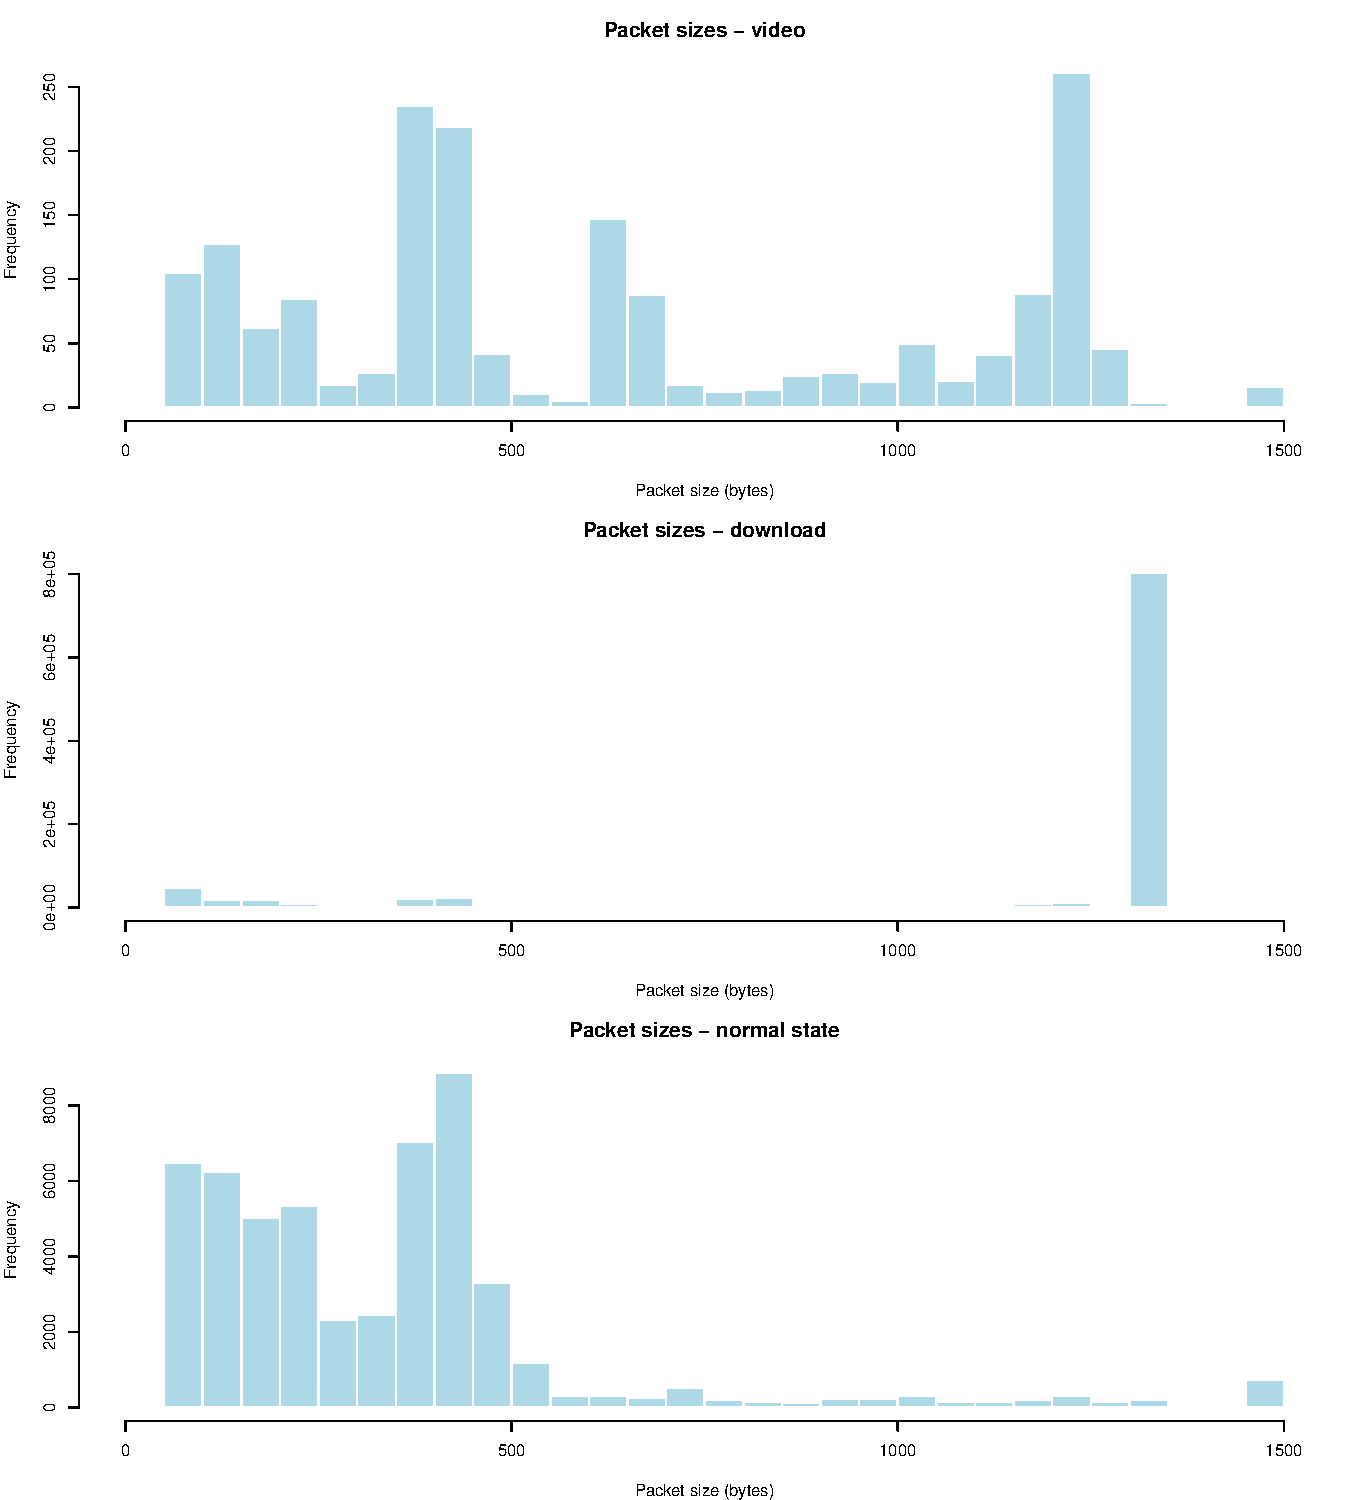
\includegraphics[width=0.82\textwidth]{../images/E9_packet_sizes.pdf}
    \caption{Packet-size histograms for the video, download, and normal-state captures, using common 50-byte bins.}
    \label{fig:ex9_packet_sizes}
\end{figure}

\textbf{Conclusion:} Video and download have similar medians (1292 and 1304 bytes), while normal-state traffic has a substantially smaller median (330 bytes). The means are 1088.96, 1121.25, and 345.21 bytes, respectively. For video and download, the median exceeds the mean, indicating that smaller packet observations pull the mean downward; in the normal-state capture the mean is slightly above the median. The 1514-byte observations are retained as recorded by Wireshark, and their presence alone is not sufficient to identify an offloading artifact. These statistics describe the captured sessions only; they do not establish that the activity itself caused the observed packet-size differences.

\subsection{Exercise 10}

\textbf{Objective:} Measure 10 Round Trip Times (RTTs) to a distant country and determine two 95\% confidence intervals for the average RTT, one based on the Student's $t$ distribution and the other on the Normal distribution, discussing which is preferable.

\textbf{Approach:} The destination, \texttt{www.uq.edu.au} (University of Queensland, Australia), was suggested by an LLM-based chatbot that was consulted for a suitable distant host; the measurements themselves were collected by us. Ten RTTs were obtained in a single run of \texttt{ping -c 10}, all of them valid replies (Figure~\ref{fig:ex10_ping}). The sample mean $\bar{x}$, standard deviation $s$ and standard error $s/\sqrt{n}$ were computed, and the critical points were obtained with \texttt{qnorm()} and \texttt{qt()}. Both intervals have the form $\bar{x} \pm c \cdot s/\sqrt{n}$, differing only in the critical value $c$: $z_{0.975}$ for the Normal and $t_{0.975,\,n-1}$ for Student's $t$.

\begin{figure}[H]
    \centering
    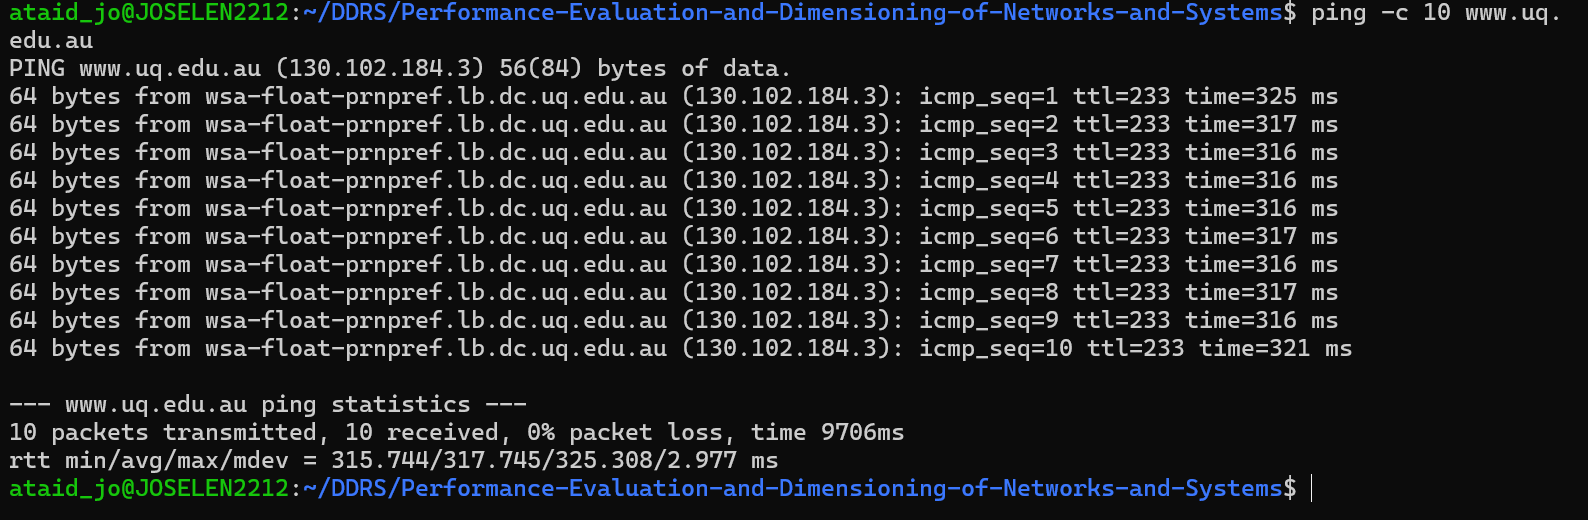
\includegraphics[width=\textwidth]{../images/ping RTTs.png}
    \caption{Output of \texttt{ping -c 10 www.uq.edu.au}.}
    \label{fig:ex10_ping}
\end{figure}

\begin{configbox}
rtt <- c(325, 317, 316, 316, 316, 317, 316, 317, 316, 321)   # RTT samples (ms)

n    <- length(rtt)
xbar <- mean(rtt)
s    <- sd(rtt)
se   <- s / sqrt(n)                          # standard error of the mean

alpha  <- 0.05                               # 95% confidence
z_crit <- qnorm(1 - alpha/2)                 # Normal critical point
t_crit <- qt(1 - alpha/2, df = n - 1)        # Student's t critical point

ci_normal <- c(xbar - z_crit * se, xbar + z_crit * se)
ci_t      <- c(xbar - t_crit * se, xbar + t_crit * se)
\end{configbox}

\begin{table}[H]
\centering
\begin{tabular}{|c|c|c|c|c|c|}
\hline
$n$ & $\bar{x}$ (ms) & $s$ (ms) & $s/\sqrt{n}$ (ms) & Critical value & 95\% CI (ms) \\
\hline
10 & 317.70 & 2.98 & 0.94 & $z = 1.960$ (Normal) & $[315.85,\ 319.55]$ \\
10 & 317.70 & 2.98 & 0.94 & $t_{9} = 2.262$ (Student) & $[315.57,\ 319.83]$ \\
\hline
\end{tabular}
\caption{95\% confidence intervals for the average RTT using the Normal and Student's $t$ distributions.}
\label{tab:ex10_results}
\end{table}

\begin{figure}[H]
    \centering
    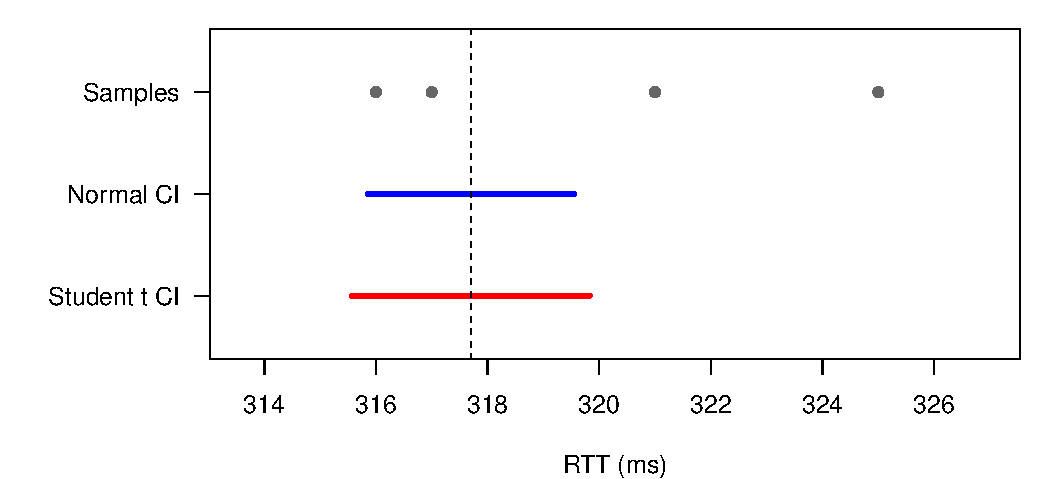
\includegraphics[width=0.75\textwidth]{../images/E10_CI.pdf}
    \caption{RTT samples and the two 95\% confidence intervals (dashed line: sample mean).}
    \label{fig:ex10_ci}
\end{figure}

\textbf{Conclusion:} As shown in Table~\ref{tab:ex10_results} and Figure~\ref{fig:ex10_ci}, the Student's $t$ interval is wider than the Normal interval (4.27~ms versus 3.70~ms), since $t_{9}=2.262 > z=1.960$. With a small sample and unknown population standard deviation, the Student's $t$ interval is generally preferable under the assumption that the observations are independent and approximately Normal. The Normal interval here uses the sample standard deviation in place of the unknown population value; its actual coverage depends on the population distribution and cannot be asserted from this sample alone. Eight observed RTTs lie between 316 and 317~ms, while 321 and 325~ms are higher. These ten measurements are not enough to establish that the underlying RTT distribution is non-Normal or right-skewed, so the shape should be treated cautiously; Exercise 11 studies interval coverage under known distributions.

\subsection{Exercise 11}

\textbf{Objective:} For four distributions -- standard Normal ($\mu=0,\sigma^2=1$), Exponential ($\lambda=1$), Lognormal ($\mu=0,\sigma^2=1$) and Lognormal ($\mu=0,\sigma^2=2$) -- and for sample sizes $n=5,10,50,5000$, estimate the coverage of the 95\% confidence interval for the mean based on 1000 experiments, and discuss whether these intervals can be trusted.

\textbf{Approach:} For each distribution and each sample size $n$, 1000 samples of size $n$ were generated. For each sample, the 95\% CI for the mean was computed as $\bar{x} \pm t_{0.975,\,n-1}\cdot s/\sqrt{n}$, using the Student's $t$ critical point, and the coverage was estimated as the fraction of the 1000 intervals that contained the true population mean $\mu$. For the exponential distribution $\mu=1/\lambda=1$, and for the lognormal distributions $\mu=e^{\,\mu_{\log}+\sigma^2/2}$, giving $\mu\approx1.649$ for $\sigma^2=1$ and $\mu\approx2.718$ for $\sigma^2=2$.

The table and figure report one Monte Carlo realization. Since the script does not set a random seed, the exact coverage estimates may differ when it is run again.

\begin{configbox}
E <- 1000                              # number of experiments
SizesOfSamples <- c(5, 10, 50, 5000)   # sizes of samples
tcritical <- qt(0.975, df = SizesOfSamples - 1)   # critical points, t distribution

# Estimates the CI coverage for one distribution
#   rgen: function(N) that generates a sample of size N
#   mu:   true (population) mean
coverage <- function(rgen, mu) {
  InInt <- rep(0, length(SizesOfSamples))
  for (i in seq_along(SizesOfSamples)) {
    N <- SizesOfSamples[i]
    for (j in 1:E) {
      a  <- rgen(N)
      ma <- mean(a)
      va <- var(a)
      alinf <- ma - tcritical[i] * sqrt(va / N)
      alsup <- ma + tcritical[i] * sqrt(va / N)
      if (mu > alinf & mu < alsup) InInt[i] <- InInt[i] + 1
    }
  }
  return(InInt / E)
}

# Standard Normal (mu = 0, sigma^2 = 1): mean = 0
cov_norm <- coverage(function(N) rnorm(N), mu = 0)

# Exponential (lambda = 1): mean = 1/lambda = 1
cov_exp <- coverage(function(N) rexp(N, rate = 1), mu = 1)

# Lognormal (mu = 0, sigma^2 = 1): mean = exp(mu + sigma^2/2)
cov_ln1 <- coverage(function(N) rlnorm(N, meanlog = 0, sdlog = 1), mu = exp(0 + 1/2))

# Lognormal (mu = 0, sigma^2 = 2)
cov_ln2 <- coverage(function(N) rlnorm(N, meanlog = 0, sdlog = sqrt(2)), mu = exp(0 + 2/2))
\end{configbox}

\begin{table}[H]
\centering
\begin{tabular}{|c|c|c|c|c|}
\hline
$n$ & Normal & Exponential & Lognormal ($\sigma^2=1$) & Lognormal ($\sigma^2=2$) \\
\hline
5    & 0.951 & 0.898 & 0.807 & 0.699 \\
10   & 0.960 & 0.899 & 0.846 & 0.746 \\
50   & 0.957 & 0.930 & 0.904 & 0.815 \\
5000 & 0.950 & 0.953 & 0.951 & 0.940 \\
\hline
\end{tabular}
\caption{Estimated coverage of the nominal 95\% confidence interval for the mean, for four distributions and four sample sizes (1000 experiments each).}
\label{tab:ex11_results}
\end{table}

\begin{figure}[H]
    \centering
    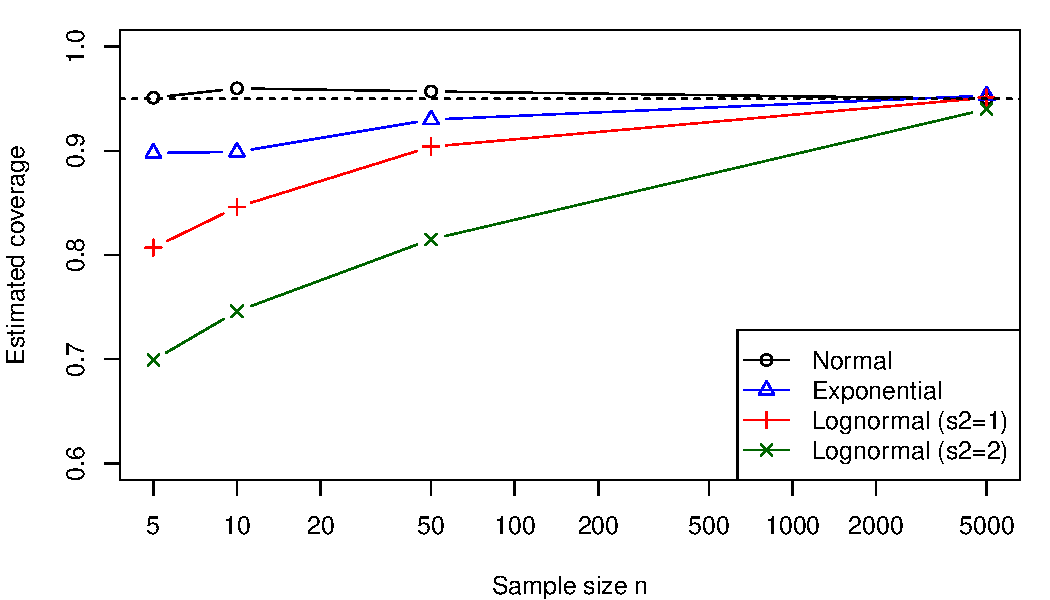
\includegraphics[width=0.8\textwidth]{../images/E11_Coverage.pdf}
    \caption{Estimated coverage vs. sample size $n$ (log scale), for the four distributions. Dashed line: nominal 95\% level.}
    \label{fig:ex11_coverage}
\end{figure}

\textbf{Conclusion:} The results illustrate that empirical coverage depends on both the sample size and the distribution. For the Normal population, the observed coverages are close to the nominal 95\% at all four sample sizes. For the skewed populations they are generally lower at small sample sizes and move closer to 95\% as $n$ increases, although the estimate at $n=5000$ for the lognormal with $\sigma^2=2$ is still 0.940. This last difference should be interpreted in light of Monte Carlo uncertainty: with 1000 experiments, an estimated coverage near 0.95 has a standard error of about 0.007. The results are consistent with the Central Limit Theorem improving the Normal approximation for larger samples, but a single set of 1000 experiments does not prove exact coverage or systematic bias.

% ======================================================================
\section{F. Output data analysis}
% ======================================================================

\subsection{Exercise 12}

\textbf{Objective:} Assess the variability of the M/M/1 average queue-delay estimate by running the simulator ten times, with 1000 completed customers per run and traffic intensity $\rho=\lambda/\mu=0.8$, and determine whether a single simulation is sufficient to draw conclusions.

\textbf{Approach:} The event-driven logic in \texttt{mm1.R} was parameterized in the Exercise 12 script because that helper is a standalone script with fixed input values. Ten independent runs used $\lambda=0.8$ and $\mu=1$, giving $\rho=0.8$. Each estimate is the accumulated queueing delay divided by the number of customers crossing the queue; customers that enter service immediately contribute zero. A fixed random seed (12) makes the experiment reproducible. The simulation loop was repeated as follows:

\begin{configbox}
set.seed(12)
queue_delay_estimates <- replicate(
    10,
    simulate_mm1_queue_delay(
        arrival_rate = 0.8,
        service_rate = 1,
        completed_customers = 1000
    )
)
\end{configbox}

The theoretical steady-state average queue delay is
\[
W_Q = \frac{\lambda}{\mu(\mu-\lambda)}
        = \frac{0.8}{1(1-0.8)} = 4.
\]
The ten simulation estimates are shown in Table~\ref{tab:ex12_runs}.

\begin{table}[H]
\centering
\begin{tabular}{|c|c||c|c|}
\hline
Run & $W_Q$ estimate & Run & $W_Q$ estimate \\
\hline
1 & 2.7141 & 6 & 2.3415 \\
2 & 4.0146 & 7 & 4.9274 \\
3 & 2.7726 & 8 & 3.4723 \\
4 & 3.7525 & 9 & 2.4955 \\
5 & 3.2918 & 10 & 3.9343 \\
\hline
\end{tabular}
\caption{Average queue-delay estimates from ten independent M/M/1 simulation runs (1000 completed customers per run).}
\label{tab:ex12_runs}
\end{table}

Across the ten replications, the sample mean was 3.3717 and the sample standard deviation was 0.8118. The estimates ranged from 2.3415 to 4.9274. A 95\% Student's $t$ confidence interval for the mean across replications was $[2.7909,\,3.9524]$, which does not contain the theoretical value $W_Q=4$; this illustrates the uncertainty remaining with only ten replications.

\begin{figure}[H]
        \centering
        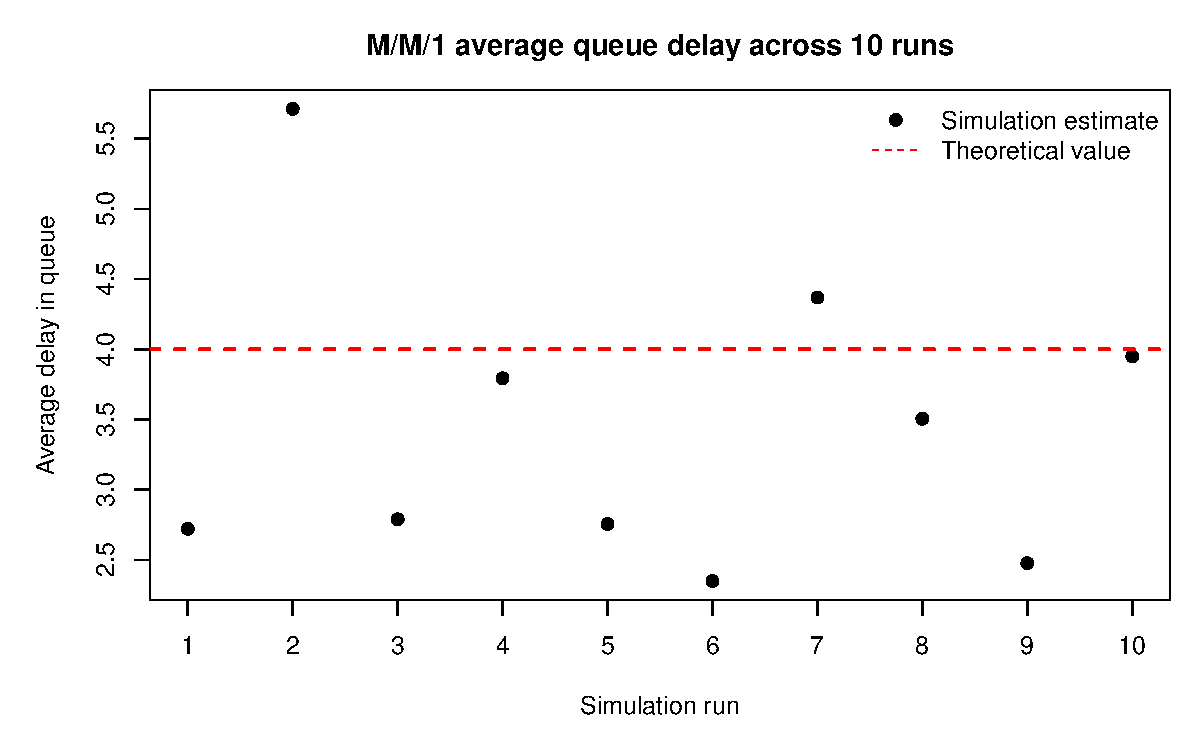
\includegraphics[width=0.78\textwidth]{../images/E12_delay_runs.pdf}
        \caption{Average queue-delay estimate in each of the ten M/M/1 runs. The dashed line marks the theoretical value $W_Q=4$.}
        \label{fig:ex12_runs}
\end{figure}

\textbf{Conclusion:} The estimates differ noticeably from run to run even though each run processes 1000 completed customers. They range from 2.3415 to 4.9274, so a single run cannot characterize the estimator's variability. The mean across the ten runs is 3.3717, and its 95\% confidence interval $[2.7909,\,3.9524]$ does not contain the theoretical value 4. This does not contradict the steady-state formula: with only ten replications, the estimate of the mean itself remains uncertain, and this particular experiment produced a low interval. More independent replications or longer runs are needed for a more stable comparison.

\subsection{Exercise 13}

\textbf{Objective:} Evaluate how the initial number of customers in an M/M/1 system affects estimates of the average delay in queue. Twenty-five independent runs were performed for each combination of run length (20 or 2000 completed customers) and initial population (0 or 10 customers), with $\lambda=3$ and $\mu=4$.

\textbf{Approach:} The supplied \texttt{fmm1\_initcond()} function in \texttt{initcond.R} was used for every run. It creates the initial population using successive exponential inter-arrival times, then simulates until the requested number of customers has crossed the queue. The four combinations of run length and initial population were generated with 25 independent replications each:

\begin{configbox}
set.seed(13)
run_results <- expand.grid(
    run = 1:25,
    run_length = c(20, 2000),
    initial_clients = c(0, 10)
)
run_results$average_queue_delay <- mapply(
    fmm1_initcond,
    ArrivalRate = 3,
    ServiceRate = 4,
    NumEndClients = run_results$run_length,
    InitClients = run_results$initial_clients
)
\end{configbox}

For $\rho=\lambda/\mu=0.75$, the theoretical steady-state mean delay in queue is
\[
W_Q = \frac{\lambda}{\mu(\mu-\lambda)}
        = \frac{3}{4(4-3)} = 0.75.
\]
Table~\ref{tab:ex13_initial_conditions} reports the mean of the 25 simulation estimates for each condition and the corresponding 95\% Student's $t$ confidence interval across replications.

\begin{table}[H]
\centering
\begin{tabular}{|c|c|r|c|}
\hline
Completed customers & Initial customers & Mean $W_Q$ & 95\% confidence interval \\
\hline
20 & 0 & 0.6183 & $[0.3648,\,0.8718]$ \\
20 & 10 & 2.2925 & $[1.9915,\,2.5935]$ \\
2000 & 0 & 0.6983 & $[0.6515,\,0.7451]$ \\
2000 & 10 & 0.7692 & $[0.6984,\,0.8399]$ \\
\hline
\end{tabular}
\caption{M/M/1 average queue-delay estimates over 25 runs per condition ($\lambda=3$, $\mu=4$).}
\label{tab:ex13_initial_conditions}
\end{table}

\begin{figure}[H]
        \centering
        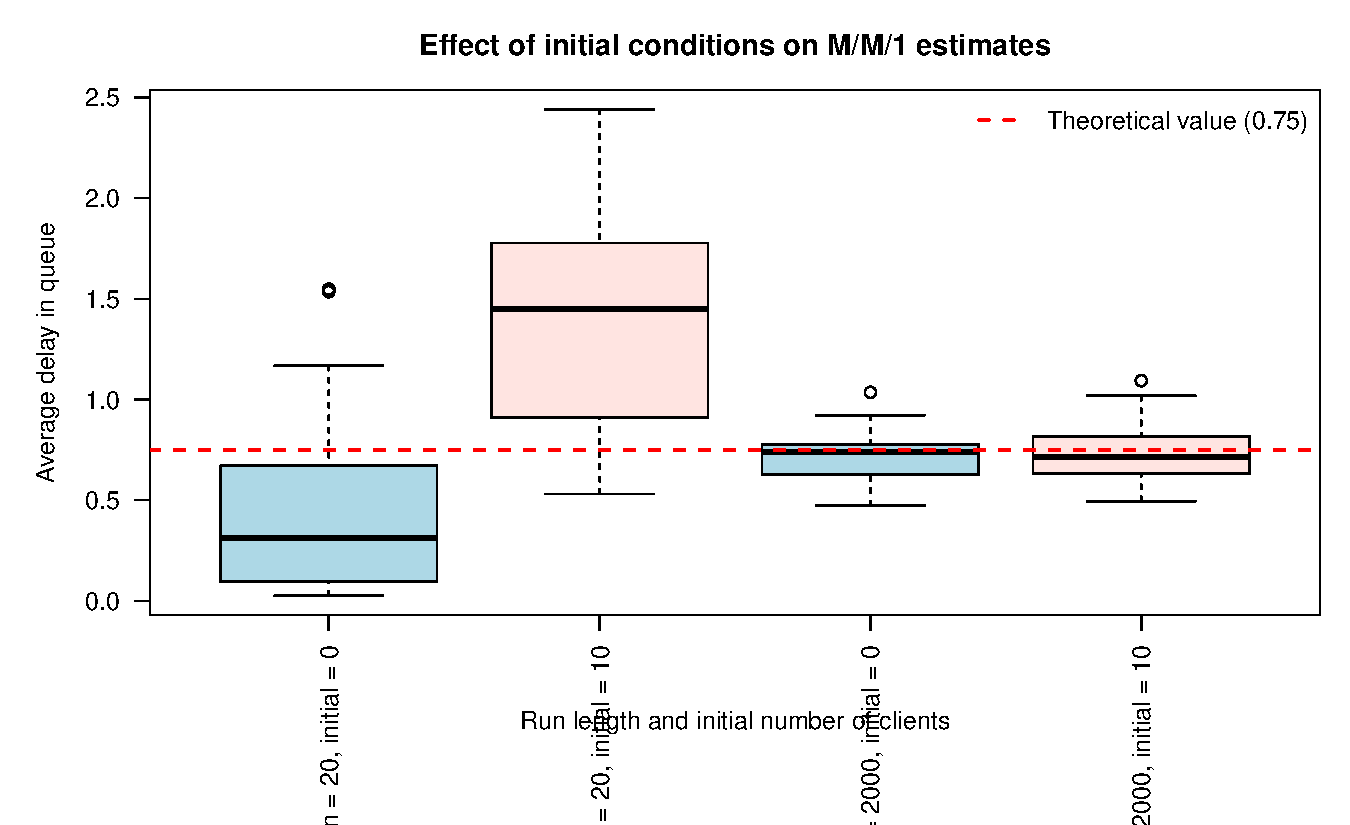
\includegraphics[width=0.88\textwidth]{../images/E13_initial_conditions.pdf}
        \caption{Distribution of the 25 average queue-delay estimates for each run length and initial condition. The dashed line marks the theoretical value $W_Q=0.75$.}
        \label{fig:ex13_initial_conditions}
\end{figure}

\textbf{Conclusion:} With only 20 customers, the initial population has a pronounced effect: the mean estimate is 0.6183 when starting empty and 2.2925 when starting with ten customers. Under the helper's initialization, the initial queue is formed through successive arrivals before the main simulation loop, so the initial waiting times strongly affect this short run. With 2000 customers, both estimates (0.6983 and 0.7692) are close to the theoretical value 0.75, and the initial-condition effect is much smaller. The confidence intervals show the same pattern: the short-run interval for ten initial customers is well above 0.75, whereas both long-run intervals include or nearly include the theoretical value (the empty-start interval ends at 0.7451). Longer runs therefore reduce, but do not eliminate in every finite sample, the initial-transient effect.

\subsection{Exercise 14}

\textbf{Objective:} Study how the number of independent replications required to estimate the M/M/1 average queue delay depends on the target relative error, the number of measured delays per replication, and the traffic intensity $\rho=\lambda/\mu$.

\textbf{Approach:} The supplied \texttt{frepdel()} function in \texttt{repdel.R} was used. It starts with ten independent replications, deletes the first 100 queue delays in each replication, and adds replications until the relative half-width of the 95\% Student's $t$ confidence interval satisfies the helper's criterion:
\[
\frac{t_{0.975,R-1}\,s_R}{\sqrt{R}\,|\bar{W}_{Q,R}|} \leq \frac{\gamma}{1+\gamma},
\]
where $R$ is the number of replications, $s_R$ is the sample standard deviation of the replication estimates, and $\gamma$ is the requested relative error. We used $\mu=1$, $\rho\in\{0.50,0.80,0.95\}$, measured sample sizes $n\in\{100,1000\}$, and $\gamma\in\{5\%,10\%,20\%\}$. The theoretical mean and variance of one steady-state M/M/1 queue delay are
\[
E[W_Q]=\frac{\rho}{\mu-\lambda}, \qquad
\operatorname{Var}(W_Q)=\frac{\rho(2-\rho)}{(\mu-\lambda)^2}.
\]
For $\mu=1$, the theoretical variances are 3, 24, and 399 for $\rho=0.50$, 0.80, and 0.95, respectively. Figure~\ref{fig:ex14_repdel} shows both this increase and the observed replication requirements.

\begin{table}[H]
\centering
\small
\begin{tabular}{|c|r|r|r|r|}
\hline
$\rho$ & Delays per replication & $\gamma=5\%$ & $\gamma=10\%$ & $\gamma=20\%$ \\
\hline
0.50 & 100 & 550 & 103 & 36 \\
0.80 & 100 & 1102 & 356 & 116 \\
0.95 & 100 & 1036 & 314 & 73 \\
\hline
0.50 & 1000 & 37 & 12 & 10 \\
0.80 & 1000 & 243 & 76 & 19 \\
0.95 & 1000 & 771 & 227 & 53 \\
\hline
\end{tabular}
\caption{Number of replications required to reach each relative-error target using a 95\% confidence interval. At least ten replications were used in every case.}
\label{tab:ex14_repdel}
\end{table}

\begin{figure}[H]
    \centering
    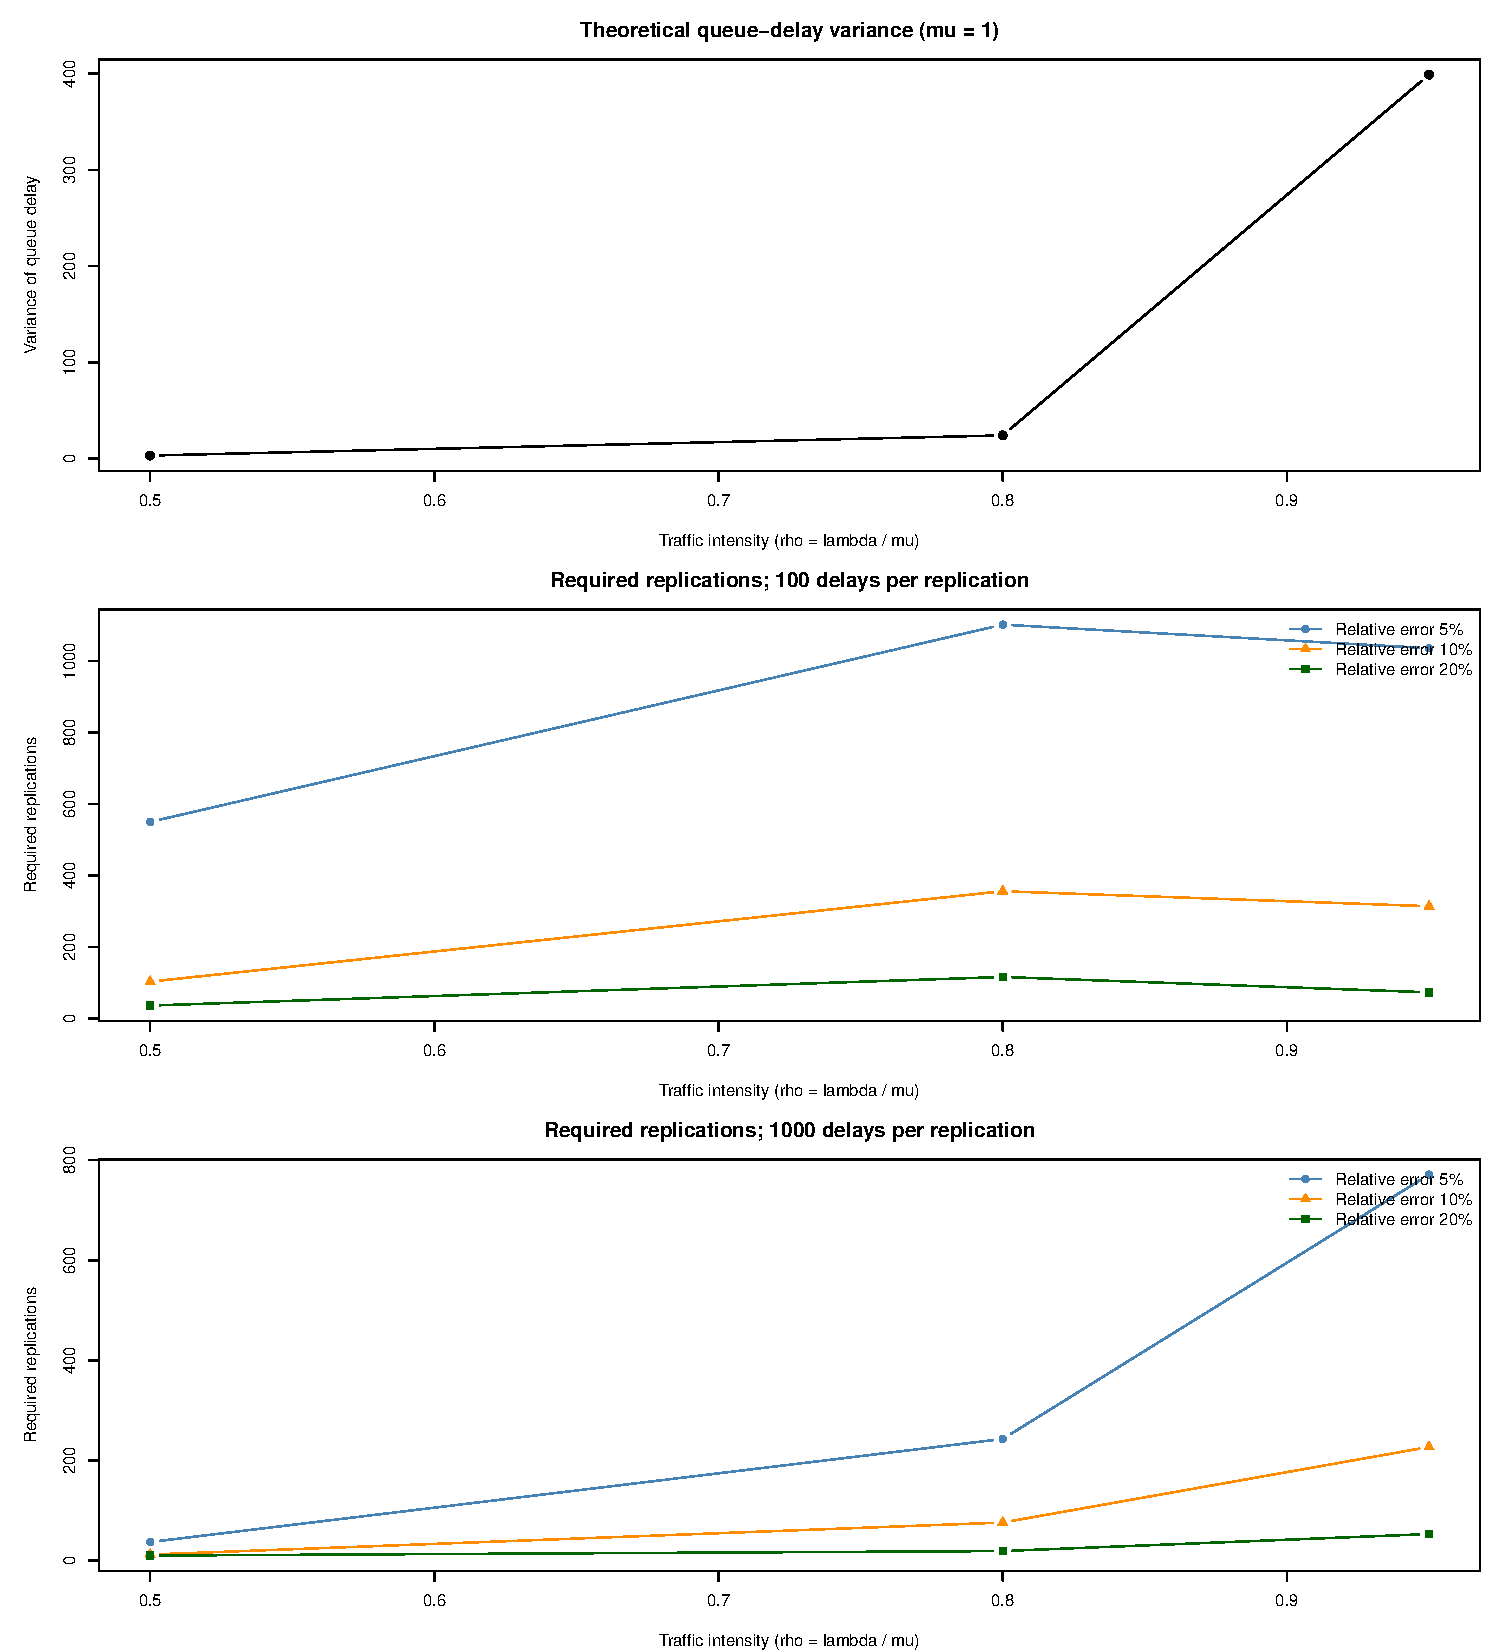
\includegraphics[width=0.82\textwidth]{../images/E14_repdel_analysis.pdf}
    \caption{Theoretical queue-delay variance and observed replication requirements as functions of $\rho$, for two measured sample sizes.}
    \label{fig:ex14_repdel}
\end{figure}

\textbf{Conclusion:} The table shows that stricter relative-error targets generally require more replications, while measuring more delays per replication generally reduces the count. Queue-delay variance increases sharply with load, from 3 at $\rho=0.50$ to 399 at $\rho=0.95$, so high-load estimates are intrinsically more variable. The measured counts are stochastic and are not monotonic in $\rho$ for every row; therefore, this experiment supports the role of variability and precision in replication effort but does not establish that the required count rises monotonically with traffic intensity in every finite run.

% ======================================================================
\section{Conclusion}
% ======================================================================

This laboratory work covered the full pipeline needed to build and validate a discrete-event simulator: generating random numbers and random variables, using them to drive event-driven simulation models, and applying statistical techniques to interpret the resulting output correctly.

Exercises 1--2 confirmed that R's random number generator is uniformly distributed yet fully deterministic given a seed, a property essential to the reproducibility of every simulation in this report. Exercises 3--5 showed that Bernoulli, exponential, and Poisson-process samples can all be derived from this single uniform generator, with their empirical distributions matching the corresponding theoretical ones.

Exercises 6--7 used these techniques to build M/M/1 and M/M/2 simulators. For stable configurations ($\rho<1$), simulated delays and utilization closely matched queuing theory, while the critically loaded case ($\rho=1$) showed that a finite simulated delay at the stability boundary does not estimate a (theoretically infinite) steady-state quantity. Comparing the two systems also illustrated the benefit of server pooling, with two parallel servers achieving lower delay than a single server of equivalent aggregate capacity.

Exercise 8 demonstrated Monte Carlo estimation of a probability, converging toward the exact binomial value as expected. Exercise 9 applied similar tools to real captured traffic, showing that bulk transfers (video, downloads) produce large, near-MTU packets, while idle traffic is dominated by small control messages.

Exercises 10--11 addressed the reliability of confidence intervals: the RTT measurements favored the more conservative Student's $t$ interval for small samples, and the coverage study quantified why, showing that intervals built from skewed distributions with small $n$ cover the true mean far less often than the nominal 95\% suggests, only becoming trustworthy once $n$ is large enough for the CLT approximation to hold.

Finally, Exercises 12--14 examined practical challenges of output analysis. Exercise 12 illustrated run-to-run variability in finite simulations. Exercise 13 showed that initial conditions can strongly affect short-run estimates, with a smaller effect in longer runs. Exercise 14 showed that replication effort depends on the precision target, the number of measured delays per replication, and the traffic intensity; the increasing theoretical queue-delay variance near saturation motivates additional replication, although the finite-run counts need not increase monotonically for every tested case.

Taken together, the exercises show that a correct simulation result depends not only on a correctly implemented model, but also on a sound statistical treatment of its output -- adequate replication, awareness of initial-transient effects, and confidence intervals appropriate to the shape of the underlying data.

\end{document}